\section{Problem \& Approach} \label{sect:overview}

\subsection{Problem Definition} \label{sect:problem}

We consider a data owner (client) storing her data in encrypted form on a server, possibly residing on a centralized cloud or a peer-to-peer (P2P) network.
The owner may run computational intensive tasks over the encrypted data.
Instead of performing tasks on the server itself, the owner delegates them to multiple workers residing on a decentralized cloud. 
Each worker fetches its portion of the required dataset from the server, performs the requested computation, and returns the results to the server.
The owner can then, at her discretion, download and verify the results.
The worker is financially rewarded if the verification of the returned results passes through.
This is illustrated in Figure~\ref{fig:model}.
In this work, we ask the question of {\em how can the owner securely and efficiently verify the resource consumption of each worker without relying on a trusted third party or any trusted hardware component}?

\begin{figure}[h!]\centering
  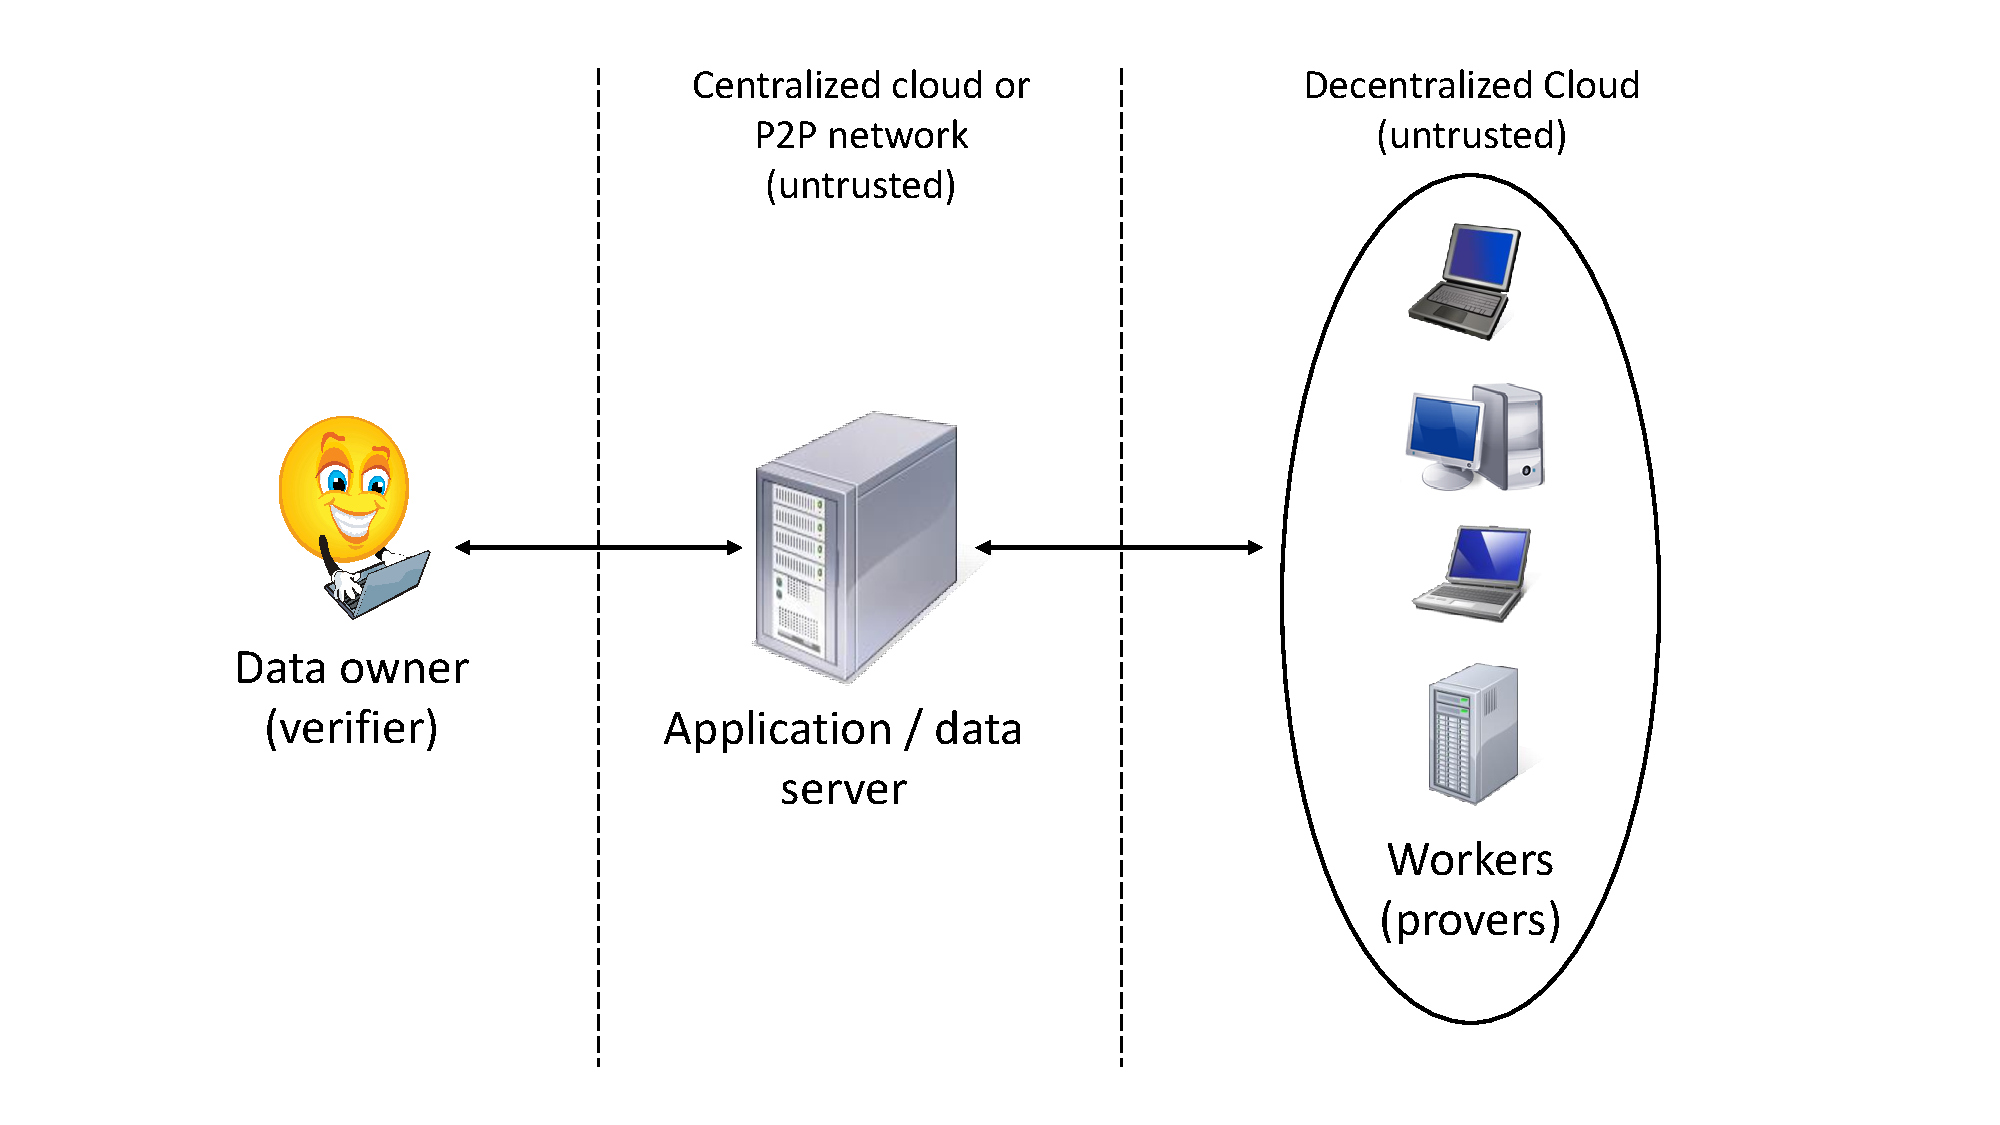
\includegraphics[scale=0.30]{model.pdf}
  \caption{Outsource of data and computation to a decentralized cloud.}
  \label{fig:model}
\end{figure}

Our decentralized cloud setting has the following distinctive characteristics in comparison to centralized cloud settings previously considered:
\begin{itemize}
 \item A data owner distributes her datasets and delegate computational tasks to a decentralized and heterogeneous computing environment.
 \item There exists an intermediate party, i.e., application/data server, which facilitates delegation and distribution of datasets and computational tasks.
 \item The owner can dynamically update her datasets stored on the server, but the data delegated to workers is assumed to be static.
 \item The owner's dataset is stored on the server over an extended period of time, but any data distributed to the worker is only temporarily stored and deleted upon the completion of the assigned task.
\end{itemize}

We note that the introduction of a centralized entity to facilitate distribution of tasks is necessary in our decentralized infrastructure.
In fact, BOINC~\cite{And04} also relies on centralized data and application servers to distribute tasks within a volunteer computing network, and BitTorrent~\cite{Coh03} uses a trusted, centralized tracker to coordinate activities within a P2P network.

\paragraph{Threat Model.}
However, each worker is assumed to be untrusted and they may deviate from the intended computation for various reasons, e.g., to save on computational cost. 
%It is essential, therefore, for the client to be able to verify the correctness of the computation. 
On the other hand, the worker may not trust the data owner either, in the sense that the worker may not be rewarded even if it has completed the computation and proved the correctness of the computation.


\subsection{Challenges} \label{sect:challenges}

\paragraph{Proofs of Data Fetch.}
- One challenge is how to reduce the number of verifications required over multiple workers (currently a prover can convince a verifier with a constant number of challenges/responses for each file). 

- Another issue is that if the worker knows in advance the positions of the challenge data blocks, then it simply downloads only those blocks. Existing POR systems do not encounter such a problem because a file is stored for a relatively extended period of time and different challenges on different positions may be issued to the worker. This forces the worker to download the entire file.

- During update of elements of the dataset, how can the owner update her local state information (used for verifying resource consumption) in an efficient manner?

\paragraph{Proofs of Computation.}


\paragraph{Fairness.}



\subsection{Solution Overview} \label{sect:solution}

